\subsection{Visualization and Analysis}
\label{sec:visualization}
In this section we describe our design goals.
We introduce the visualization module to show common and abnormal movement patterns discovered by the data analysis module.
To illustrate our method, we use the Tweets generated near the finish line of the Boston Marathon during first 24 hours after the two explosions on April 15, 2013.

\subsubsection{Design Rationale}
Our design goal is to show trajectories extracted from geo-tagged Tweets of each person.
Displaying the trajectories without grouping can also reveal new insights when users drill down to individual movements.
%A spatiotemporal filter are also required to focus on a specific spatiotemporal space.
However, when the number of trajectories shown over the map increases, visual clutter issues arise that hinder the discover of flow patterns.
To reduce clutter, we use a modified partition-based trajectory clustering model for discovering common sub-trajectory patterns~\cite{Lee:2007:Trajectory}.
%Since our trajectories are usually sparse and incomplete compared to ones generated by GPS devices (the interval is couple of seconds between each point), we need a diff
%However, clustering trajectories as a whole cannot discover similar portions of trajectories.
%Even though some portions of trajectories with a long path show a common behavior, the whole trajectories might not.
%The common sub-behavior is also valuable information.
The discovered common movements have multiple attributes to be analyzed, such as cluster size, direction, and length.
%These attributes need to be displayed.
The users need to not only identify abnormal movement patterns, but also understand how abnormal and normal movement patterns differ.
The required clustering level can also vary with the application.
So, we need to allow the users to adjust the clustering level.
%We also would like to display change of movement patterns over time.

\subsubsection{Visualization of Common Movements}

Figure~\ref{fig:clustering_process} shows the process of discovering common movement patterns.
If we display the raw trajectories, it is difficult to understand the realistic movement patterns because of the high degree of sparseness of the trajectories as shown in Figure~\ref{fig:clustering_process} (left).
Therefore, we reduce the sparseness of the raw trajectories using the method described in Section~\ref{sec:trajectory_extraction} and display the supplemented trajectory on the map with 30\% opacity in Figure~\ref{fig:clustering_process} (center).
%the trajectories with a higher opacity represent the routes used by a higher number of people.
%The supplemented trajectories represent more realistic human mobilities than the raw one.
Users are able to examine more realistic human mobilities with the supplemented trajectories rather than using the raw ones.
%The trajectories supplemented with route directions show more realistic trips (transparent yellow poly lines)  and enable users to examine individual movements, in which the lines with a higher opacity represent the routes used by a higher number of people.
%The users are able to intuitively select a specific area and a time period to focus on their interest.
%However, if the number of trajectories shown over the map increase, the users will encounter difficulty in analyzing movement patterns.
Next, we cluster the trajectories into sets of similar sub-trajectories and generate representative trajectories for each cluster as described in Section~\ref{sec:common_movement_discovery}.
The representative trajectories represent common movement behaviors in Figure~\ref{fig:clustering_process} (right).

\begin{figure}[hbt]
\centering
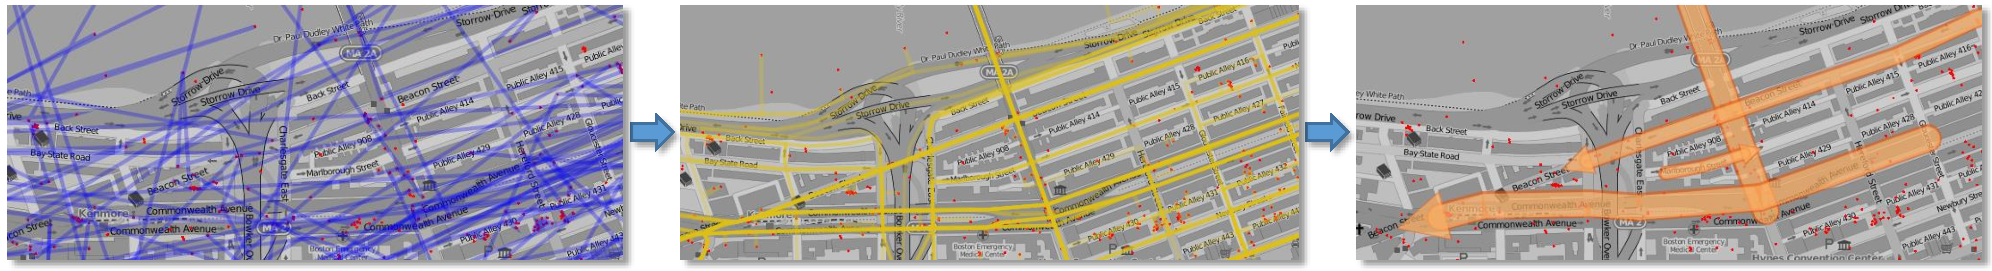
\includegraphics[width=1.0\linewidth]{clustering_process_v4}
\caption{The process of discovering common human movement patterns using location-based social networks data.
Visualization of sub-trajectory clusters (right). The thickness of each trajectory represents the size of the cluster.}
\label{fig:clustering_process}
%\vspace{-0.4cm}
\end{figure}

We provide visual cues to show multiple attributes for a representative trajectory.
We use a poly line with an arrow head to display the length and the direction of the representative trajectory.
The thickness of the line represents the size (i.e., the number of sub-trajectories belonging to a cluster) of the corresponding cluster.
Figure~\ref{fig:cluster_properties} shows the representative trajectories within the region same as the one in Figure~\ref{fig:clustering_process} (right).
Placement order of the trajectories depends on the length; the longest trajectory is placed at the bottom and the shortest one at the top, to avoid obscuring the shorter trajectories.

Our system also enables users to adjust and refine the $\epsilon$ (as neighborhood distance) and $MinLns$ (as minimum cluster size) values used by the clustering algorithm depending on their requirements by visual inspection.
We display an initial clustering result calculated with the automatically estimated parameter values as described in Section~\ref{sec:common_movement_discovery}.
The optimal result in Figure~\ref{fig:clustering_level} (top) is achieved at $\epsilon=25$ and $MinLns=3$.
The algorithm generates a larger number of smaller clusters, when $\epsilon$ is smaller or $MinLns$ is larger compared to the optimal values.
In contrast, the algorithm generates a smaller number of larger clusters when $\epsilon$ is larger or $MinLns$ is smaller.
For example, the result at $\epsilon=25$ and $MinLns=4$ is shown in Figure~\ref{fig:clustering_level} (center) and the results at $\epsilon=30$ and $MinLns=2$ is shown in Figure~\ref{fig:clustering_level} (bottom).

\begin{figure}[tb]
	\centering
	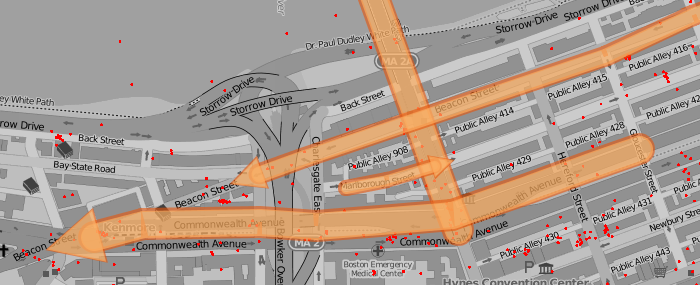
\includegraphics[width=1.0\linewidth]{Cluster_Properties}
	\caption{Visualization of sub-trajectory clusters. The thickness of each trajectory represents the size of the cluster.
	}
	\label{fig:cluster_properties}
	%\vspace{-0.4cm}
\end{figure}


\begin{figure}[tb]
	\centering
	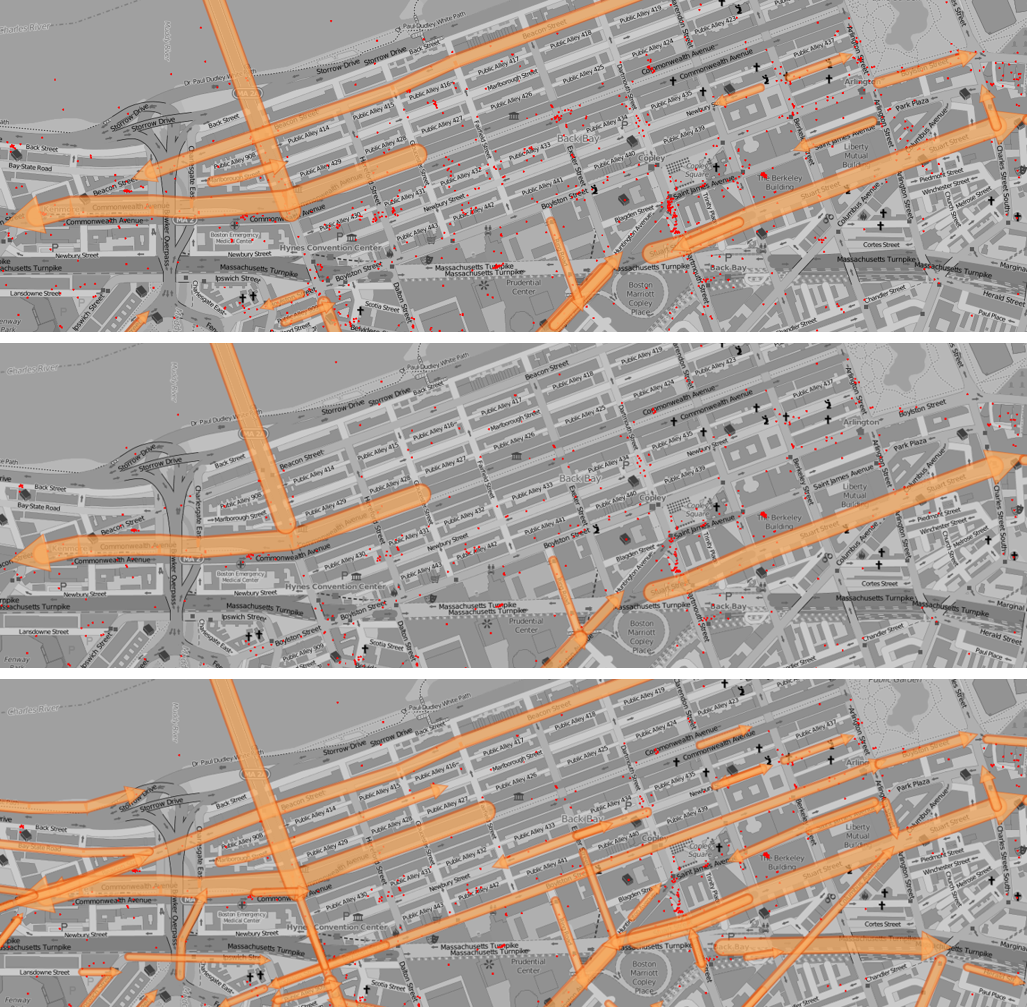
\includegraphics[width=1.0\linewidth]{clustering_level_v4}
	\caption{Clustering results depending on two parameters: $\epsilon$ and $MinLns$.
	Top ($\epsilon=25$, $MinLns=3$) is optimal.
	Center ($\epsilon=25$, $MinLns=4$) shows less number of trajectory clusters. Bottom ($\epsilon=30$, $MinLns=2$) shows more.
	}
	\label{fig:clustering_level}
	%\vspace{-0.4cm}
\end{figure}

%\subsection{Allow Customized Area Selection for Regional Trajectory Analysis}
%\subsection{Interaction}
%
%The system allows user to filter and display clusters related to a user select area. This feature allows user to select a specific polygonal area of interest and find trajectory clusters based on the trajectories that go through, go into or go out of that area.
%
%By implementing a mouse listener in Java, mouse movement and clicks can be tracked to both visualize and calculate the area has been chosen. Then each trajectory's joint points are tested to see if it lies within the selected area. If so, the trajectory is included in the selected trajectories. If a user chooses to calculate trajectory clusters under the selected area mode, the selected trajectories will be used to perform the clustering calculation. 

\begin{figure}[hbt]
	\centering
	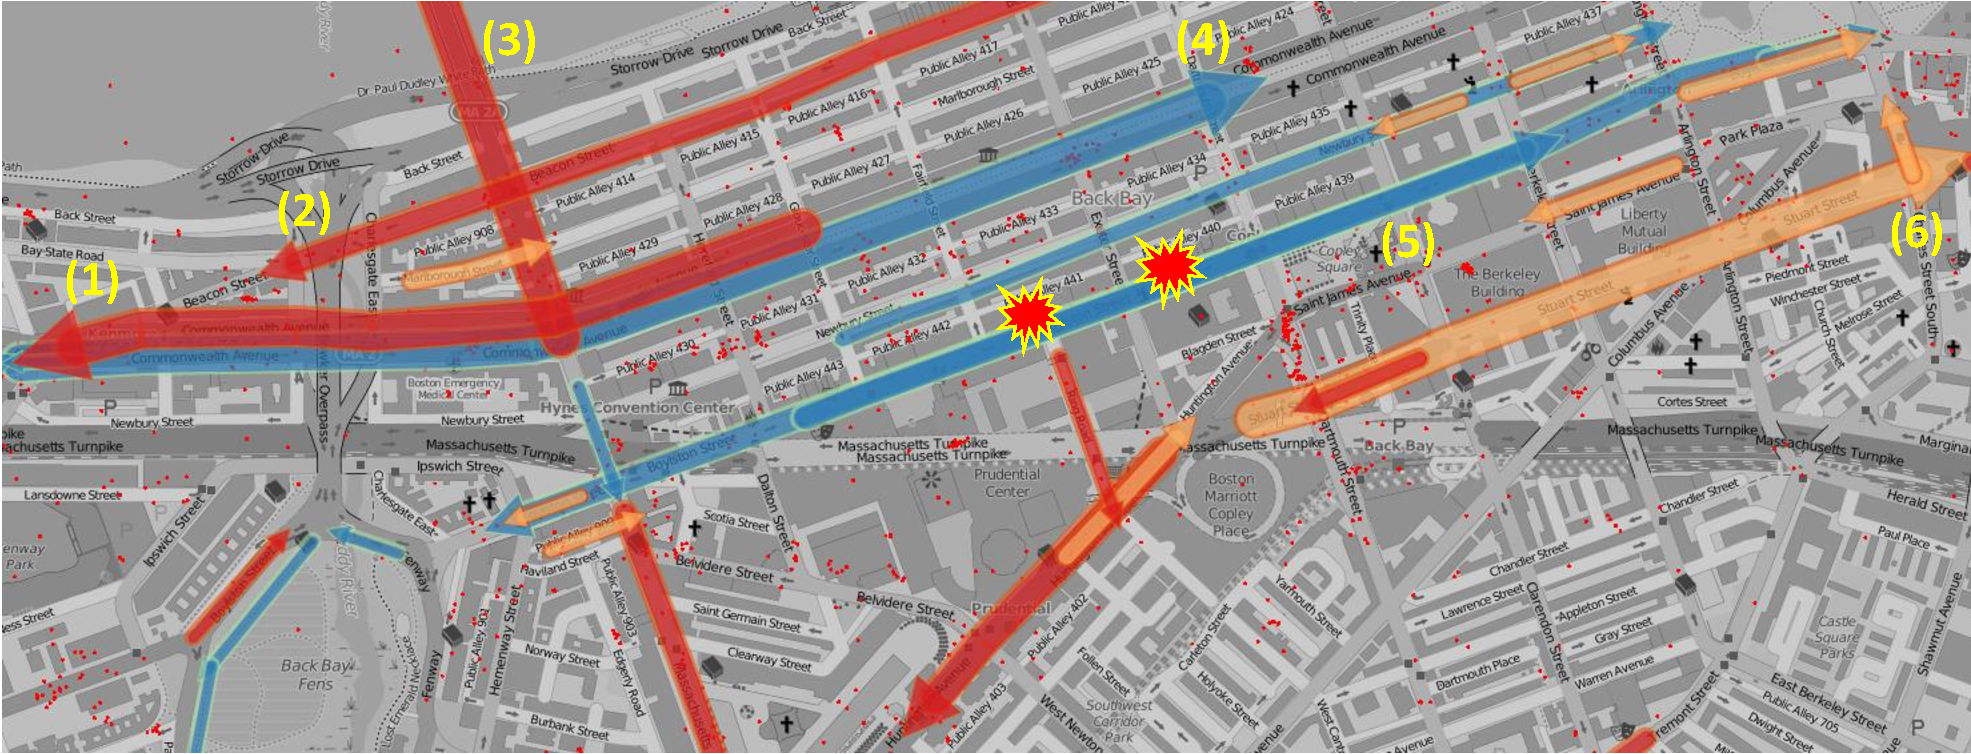
\includegraphics[width=1.0\linewidth]{abnormal_movements_v4}
	\caption{
	The trajectories (red and orange) shows the human movement patterns around the finish line at the Boston Marathon 2013 during 2 hours after the explosions.
	The trajectories (blue) represent the movements for the normal situation (the same time period of the same event in 2014).
	The two markers indicate the locations of the two explosions.
	}
	\label{fig:abnormal_movements}
	%\vspace{-0.4cm}
\end{figure}

\subsubsection{Visualization of Abnormal Movements}
\label{sec:visualization_abnormal}
Our analytics model identifies abnormal representative trajectories from target ones by comparing with normal ones as described in Section~\ref{sec:abnormal_movement_detection}.
We define target outliers are the abnormal representative trajectories and target normal trajectories are the rest of the target representative trajectories; the target normal trajectories are close to the normal representative trajectories.
We visualize the three different types of representative trajectories: target outlier, target normal, and normal using a similar visual encoding scheme described in the previous section.
We use different colors to distinguish between the different types: target outlier with red, target normal with orange, and normal with blue as shown in Figure~\ref{fig:abnormal_movements}.
%Figure~\ref{fig:abnormal_movements} shows an example case.
We can see that the trajectories (1), (2), and (3) are close to the normal trajectory (4), but they head toward the opposite direction.
Those are, therefore, classified as outliers.
The trajectory (6) is not classified as an outlier, because it is close to the normal trajectory (5) and also has the same direction.
We also provide an option to turn on/off each type to focus on a specific type.




